\documentclass[12pt]{ucsddissertation}
% mathptmx is a Times Roman look-alike (don't use the times package)
% It isn't clear if Times is required. The OGS manual lists several
% "standard fonts" but never says they need to be used.
\usepackage{mathptmx}
\usepackage[NoDate]{currvita}
\usepackage{array}
\usepackage{tabularx}
\usepackage{booktabs}
\usepackage{ragged2e}
\usepackage{microtype}
\usepackage[breaklinks=true,pdfborder={0 0 0}]{hyperref}
\usepackage{graphicx}
\usepackage{subcaption}
\usepackage{amsmath}
\usepackage{enumitem}
\usepackage{arydshln}
\AtBeginDocument{%
	\settowidth\cvlabelwidth{\cvlabelfont 0000--0000}%
}

%commands

\newcommand{\sword}{SwordBox}
\newcommand{\thesistitle}{Disaggregated Data Structures: Sharing and Contention with RDMA and Programmable Networks}

\usepackage{multirow}
\usepackage{tikz}
\newcommand*\nullcirc[1][1ex]{\tikz\draw (0,0) circle (3pt);} 
\newcommand*\halfcirc[1][1ex]{%
  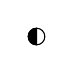
\begin{tikzpicture}
  \draw[fill] (0,0)-- (90:3pt) arc (90:270:3pt) -- cycle ;
  \draw (0,0) circle (3pt);
  \end{tikzpicture}}
\newcommand*\fullcirc[1][1ex]{\tikz\fill (0,0) circle (3pt);} 

% OGS recommends increasing the margins slightly.
\increasemargins{.1in}

% These are just for testing/examples, delete them
\usepackage{trace}
%\usepackage{showframe} % This package was just to see page margins
\usepackage[english]{babel}
\usepackage{blindtext}
\input{annotations}
\overfullrule5pt
% ---

% Required information
\title{\thesistitle}
\author{Stewart Steven Grant}
\degree{Computer Science}{Doctor of Philosopy}
% Each member of the committee should be listed as Professor Foo Bar.
% If Professor is not the correct title for one, then titles should be
% omitted entirely.
\chair{Professor Alex C. Snoeren}
% Your committee members (other than the chairs) must be in alphabetical order
\committee{Professor Amy Ousterhout}
\committee{Professor George Papen}
\committee{Professor Yiying Zhang}
\degreeyear{2024}

% Start the document
\begin{document}
% Begin with frontmatter and so forth
\frontmatter
\maketitle
\makecopyright
\makesignature
% Optional
\begin{dedication}
\setsinglespacing
\raggedright % It would be better to use \RaggedRight from ragged2e
\parindent0pt\parskip\baselineskip

\textit{To my inner circle -- Family, Loved ones and Friends. And to every belayer that caught me. Thanks for the proverbial and literal support.}


% In recognition of reading this manual before beginning to format the
% doctoral dissertation or master's thesis; for following the
% instructions written herein; for consulting with OGS Academic Affairs
% Advisers; and for not relying on other completed manuscripts, this
% manual is dedicated to all graduate students about to complete the
% doctoral dissertation or master's thesis.

% In recognition that this is my one chance to use whichever
% justification, spacing, writing style, text size, and/or textfont that
% I want to while still keeping my headings and margins consistent.
\end{dedication}
% Optional
\begin{epigraph}
\vskip0pt plus.5fil
\setsinglespacing
{\flushright

"If this is the best of possible worlds, what then are the others?"\\
\vskip\baselineskip
-Voltaire \textit{Candide}\par}

\vfil
\begin{center}

\noindent “It must be considered that there is nothing more difficult to carry out, nor more
doubtful of success, nor more dangerous to handle, than to initiate a new order of things.”

\vskip\baselineskip
\hskip0pt plus1fil -Niccolo Machiavelli \textit{The Prince}\hskip0pt plus4fil\null

\end{center}
\vfil
"If every porkchop were perfect we wouldn't have hotdogs"\\

\vskip\baselineskip
-Greg Universe, \textit{Steven Universe}

\vfil
\end{epigraph}

% Next comes the table of contents, list of figures, list of tables,
% etc. If you have code listings, you can use \listoflistings (or
% \lstlistoflistings) to have it be produced here as well. Same with
% \listofalgorithms.
\tableofcontents
\listoffigures
\listoftables

% Preface
% \begin{preface}
% \todo{Write a preface - take a look at some examples because it seems rather free form}
% Almost nothing is said in the manual about the preface. There is no
% indication about how it is to be typeset. Given that, one is forced to
% simply typeset it and hope it is accepted. It is, however, optional
% and may be omitted.
% \end{preface}

% Your fancy acks here. Keep in mind you need to ack each paper you
% use. See the examples here. In addition, each chapter ack needs to
% be repeated at the end of the relevant chapter.
\begin{acknowledgements}

I would like to acknowledge my advisor Alex C. Snoeren for his dedication to his craft and guidance
over the past 6 years. No piece of work within this dissertation would be possible without your
collaboration. I would also like to thank my committee members Amy Ousterhout, Yiying Zhang, and
George Papen for their feedback and guidance, and Srikanth Kandula for his mentorship during my time
at MSR.

This dissertation has been extraordinarily influenced by Anil Yelam, my closest collaborator. Thank you
for all the time you spent working on our collaborations, and the hours spent discussing and
debating system designs and performance results. I'm forever grateful. To Maxwell Bland, your
research energy is unmatched and without your help we would never have have acquired any SmartNICs.
And Alex (Enze) Liu for his superior knowledge of Python and unmatched focus on research.  Thank you
to all of the members of the Systems and Networking group at UCSD, especially the optical networking
group for your feedback and guidance during the first years of my PhD.

Thank you to Meta for funding my research and providing me with the opportunity to work on resource
disaggregation, Cavium for the generous donation of two SmartNICs, and to ARPAe for funding my first
years of research.

I'd like to thank all of the members of 3140 for their collaboration and friendship over the years.
It's truly the best office, Chez bob volunteers for keeping me fed, and to my friends for the
support. Camille Rubel thanks for having the best climbing schedule in the world, Phillip Arndt for
pushing my limits, and Camille Moore for keeping me on my toes.
\todo{double check I thanked everyone}


\end{acknowledgements}

% Stupid vita goes next
\begin{vita}
\noindent
\begin{cv}{}
\begin{cvlist}{}
\item[2012-2016] Bachelor of Science, Computer Science University of British Columbia
\item[2016-2018] Master of Science, Computer Science University of British Columbia
\item[2018-2024] Doctor of Philosophy, Computer Science University of California San Diego
\end{cvlist}
\end{cv}

% This puts in the PUBLICATIONS header. Note that it appears inside
% the vita environment. It is optional.
\publications

\noindent Deepak Bansal and Gerald DeGrace and Rishabh Tewari and Michal Zygmunt and James Grantham
and Silvano Gai and Mario Baldi and Krishna Doddapaneni and Arun Selvarajan and Arunkumar Arumugam
and Balakrishnan Raman and Avijit Gupta and Sachin Jain and Deven Jagasia and Evan Langlais and
Pranjal Srivastava and Rishiraj Hazarika and Neeraj Motwani and Soumya Tiwari and Stewart Grant and
Ranveer Chandra and Srikanth Kandula. 2023. Disaggregating Stateful Network Functions. In
proceedings of 20th USENIX Symposium on Networked Systems Design and Implementation (NSDI 23).
Usenix Association, Boston MA, USA, 1469--1487.
https://www.usenix.org/conference/nsdi23/presentation/bansal \\

\noindent Stewart Grant, Anil Yelam, Maxwell Bland, and Alex C. Snoeren. 2020. SmartNIC Performance
Isolation with FairNIC: Programmable Networking for the Cloud. In Proceedings of the Annual
conference of the ACM Special Interest Group on Data Communication on the applications,
technologies, architectures, and protocols for computer communication (SIGCOMM '20). Association for
Computing Machinery, New York, NY, USA, 681–693. https://doi.org/10.1145/3387514.3405895 \\

\noindent Stewart Grant, Hendrik Cech, and Ivan Beschastnikh. 2018. Inferring and asserting
distributed system invariants. In Proceedings of the 40th International Conference on Software
Engineering (ICSE '18). Association for Computing Machinery, New York, NY, USA, 1149–1159.
https://doi.org/10.1145/3180155.3180199 \\


% This puts in the FIELDS OF STUDY. Also inside vita and also
% optional.
% \fieldsofstudy
% \noindent Major Field: Computer Science
\end{vita}

% Put your maximum 350 word abstract here.
\begin{dissertationabstract} 
%%	
Resource disaggregation proposes a next-generation architecture for data center resources. System
components like compute, memory, storage, and accelerators are separated from one another by a fast
network and composed dynamically into virtual servers when required. This paradigm promises tyo
dramatically improved resource utilization, scalability, and flexibility, but introduces substantial
challenges in terms of performance and fault tolerance. Memory is among the most difficult resources
to disaggregate. CPUs currently expect DRAM to have ultra low latency, high bandwidth, and to share it's
failure domain. In particular increased latency from network round trips dramatically shifts the
performance of existing shared data structures designed for local DRAM.

In this dissertation I explore the challenges of sharing disaggregated memory with hundreds of CPU cores.
First in {\sword} I present a system which utilizes a centralized programmable switch to cache data
structure state and dramatically improve key-value workload performance. Second I present a new
key-value store RCuckoo which is designed to leverage RDMA and reduce round trips when accessed by
CPUs over a network. Both systems demonstrate significant performance improvements over the
existing state of the art.

\end{dissertationabstract}

% This is where the main body of your dissertation goes!
\mainmatter

% Optional Introduction
\begin{dissertationintroduction}

\textit{What should a data center server look like?} 20 years ago a data center operator may have
argued for the simplicity of homogeneity over optimal performance, reasoning that carefully picked
hardware at a given price point would yield the best cost-performance tradeoffs and that the
performance yields of next generation hardware would quickly erase any gains made by specializing
servers~\todo{cite}. 
%%
Since then both Moore's law and Dennard scaling have slowed down dramatically. CPU clock speeds and
memory density improvements have stagnated leaving operators to fight tooth and claw to enjoy the
efficiency gains of prior decades. The effect is that new technologies are being introduced to to
achieve scaling.  CPUs are now monstrously parallel. Custom accelerators are common for specialized
workloads like video coding and machine learning. Indeed the modern data center is a hodgepodge of
heterogeneous hardware (GPU's, TPU's, DPU's, SmartNICs and
FPGA's)~\cite{dsnf,azure-smartnic,tpu,nitro}, and various new memory offerings and tiers like
NVMe~\cite{decible}.  Today the number of server types in a data center, conservatively, is in the
dozens.  At the time of writing EC2 has 84 listed instance types~\cite{ec2-offer} for their
customers to design their services. The trend is clear: in search of efficiency data center and
server design is increasingly heterogeneous with servers being designed for specific applications
and workloads.

Resource disaggregation is a new architectural paradigm for data center resources aimed at improving
efficiency and managing increased heterogeneity. In the disaggregated model a server's resources do
not monolithicly reside in a 1, 2, or 4U server form factor, instead each resource, i.e compute,
memory, storage is deployed separately to a dedicated machine and interconnected via a fast network.
Servers are composed dynamically from these resources which enables them to be provisioned for their
exact purpose~\cite{dis-and-app,infiniswap,blade-server,decible,legoos}. This model enables resource
pooling and sharing which in turn leads to higher efficiency~\cite{regions,fastswap,dsnf,aifm,supernic,ditto}.

% DRAM in particular has quickly become a precious resource in the data center. Main memory capacity,
% while growing has not kept up with CPU core counts. The result is that per-core memory capacity is
% less than 10 years ago~\cite{micron-memorywall}. New memory tiers like NVMe have been introduced to
% help alleviate memory pressure from applications, but the composition of these memory tiers, and the
% software to manage them are still undecided.

DRAM in particular has become a precious resource in data centers and is a focused target for
resource pooling~\cite{micron-memorywall}. The benefits of pooling are clear when examining a simple
bin packing problem. Consider two servers both provisioned with 4GB of DRAM and three jobs each of
which requires 2.5GB of memory. In a monolithic design a scheduler can only place one job per
machine or risk swapping to disk. In a disaggregated model the 4GB of memory could be placed in an
8GB pool which could be easily subdivided into 3 2.5GB partitions. In the monolithic case the unused
memory is stranded, while pooling reclaims stranded memory.  More concretely at data center levels
practitioners have to provision their servers for the sum of peak demand, when resources are pooled
they can be provisioned for the peak of the sum of demand which can be significantly
lower~\cite{supernic, dsnf}.

Disaggregation is only possible because of new fast networks. Commodity NICs now offer 400Gbps with
expectations for continued growth, and network devices are increasingly programmable with multiple
vendors offering programable SmartNICs, DPUs and switches.  These two trends have lead to intra rack
latencies of 1-2{$\mu$}s and network bandwidths on the same order as memory bandwidths with the
ability to inspect, cache, and modify packets in flight at line rate.

Storage has seen widespread disaggregation. The key enabling factor is that storage device access
latency is far higher than a network round trip. In the case of memory the opposite is true. Memory
access latency is 20x lower than an RTT effectively making it a separate tier of memory when placed
across a network.  This performance gap plays out in dramatic fashion when porting data structures
designed for local memory to far memory systems. Sharing data between multiple remote machines where
coherence between remote cores is required leads to abysmal performance degradation (300x tail
latencies in some cases)(Chapter~\ref{chap:swordbox}). Further complicating the design of shared
data structures is that memory, once in a single fault domain, can fail ripping a hole directly into
a processes address space~\cite{amanda-hotnets,hydra,legoos}.

This dissertation explores the design of shared data structures in disaggregated memory systems.  I
present two systems ({\sword} and RCuckoo) which focus on the challenges of sharing and contending
access to remote memory. {\sword} (Chapter~\ref{chap:swordbox}) is a middlebox approach for removing
contention from shared data structures. The high level insight behind {\sword} is to leverage the
fact that at rack-scale TORs have a serialized view of traffic to and from servers. Using this idea
{\sword} caches data structure state on a programmable switch. 
%%
Second I present RCuckoo (Chapter~\ref{chap:rcuckoo}) a fully disaggregated key-value store. RCuckoo
is specially designed to improve key-value locality. Using locality sensitive hashing RCuckoo
improves reads, writes, locking and fault recovery performance by reducing the overall number of
round trips required for each operation.
%%
{\sword} yields orders of magnitude improvements in both
throughput (up to 30x) and tail latency (up to 300x).  RCuckoo meets or exceeds the performance of
all state-of-the art disaggregated key-value stores on small key-value pairs and significantly
outperforms other systems on read-mostly workloads.

\end{dissertationintroduction}

\chapter{Background}

Calls for distributed memory systems have been made for decades~\todo{define distributed memory
systems earlier}, and the groundwork of disaggregation relies heavily on the work of the
past~\cite{treadmarks,gms}. However, disaggregation differs from prior distributed systems due to
its scale and system assumptions. 
%%
Disaggregation assumes that each resource be stand alone, or paired with a miniscule amount of other
resources. For instance a storage server may have a small amount of compute such as an ARM core or
two in order to boot, configure and occasionally execute management tasks. Similarly compute servers
(CPU, GPU) are outfit with a small amount of memory (e.g 4GB~\cite{legoos}) for caching.
This assumption transforms the technologies and requirements for disaggregated systems.

\todo{add forward pointers to the rest of the background and expand this section and explain the
purpose of this chapter.}
% Critically Remote Direct Memory Access (RDMA) (or a similar CPU bypass technology) is essential in
% constructing a passive storage system.\todo{foreshadow 1.3 and 1.4 to hel}

\section{Disaggregation}

As with many paradigm shifts within the systems community the idea of disaggregation is born from
shifting hardware trends. Per-core access to memory have been decreasing for decades. CPU core
counts have consistently increased for over a decade while memory speeds and capacity have improved
comparatively slowly~\cite{micron-memorywall}. The result is that CPU cores have less access to
memory bandwidth and capacity now than 10 years ago. Memory is an increasingly scarce resource and
data center operators are exploring new ways to achieve better memory utilization.  Disaggregation
is one such option. Monolithic servers have a fixed amount of RAM per machine which, at a data
center level, leads to a skewed distributed of memory utilization.  Some servers are starving for
memory while others have gigabytes to spare. This spare (stranded) memory is one target of
disaggregation, it aims to give each server access to a shared pool of RAM.  In general a
disaggregated resource, be it memory, FPGA's, or the network itself, can be provisioned for the
peak-of-sums, rather than monolithic resources which are provisioned for the
sum-of-peaks~\cite{clio,supernic,dsnf}.

The biggest barrier to disaggregation is network latency~\cite{requirements}, and more aptly the
difficulty of disaggregating a resource is proportional to its access latency with respect to the
additional latency of the network. Disaggregated storage is a foregone conclusion. Academia and
industry have pooled SSD's and HDD's into shared storage pools for their increased capacity and
lower cost. This is relatively easy in comparison to memory as the access cost of storage is already
high relative to the network. In concrete terms intra-rack RDMA ping latencies are on the order of
1-2 us. HDD latencies are 10-20ms and SSD are often 100's of us. In these cases the network overhead
is a single digit percentage or less~\cite{decible}. In contrast DRAM latencies are 50-100ns. DRAM
over RDMA has a nearly 20x overhead compared to local access. Despite this overhead RDMA is one of
the strongest contenders for a disaggregated transport.  CXL is a burgeoning technology which
promises NUMA-like latencies (200-300ns) for remote memory access~\cite{cxl}. At the time of writing
CXL is not widely available and its performance and scalability are not well
understood~\cite{direct-cxl,pond,cxl-demyst}. Regardless of interconnect
the principle of access latency remains the same. This dissertation focuses on RDMA although we see
the algorithms and data structures presented here to be largely interconnect independent.


\section{RDMA}

Remote direct memory access (RDMA) is the key enabling technology for disaggregation. This section
describes RDMA's characteristics with respect to how it enables disaggregated architectures via its
one-sided verbs, as well as the complexities of building shared data structures on top of RDMA with
respect to serialization.

RDMA is a low latency, high bandwidth network protocol. It achieves high performance by bypassing
multiple overheads common to a traditional networking stack (e.g.  Linux Sockets). 
%%
Firstly RDMA is a kernel-bypass technology. It allows userspace applications to directly interact
with the network interface card (NIC) taking advantage of NIC specific features like on-nic
caches~\cite{sherman} and avoiding context switch overheads.
%%
Second, RDMA's most distinguishing feature is that it offloads much of the network stack to the NIC
hardware and bypasses the CPU entirely for data transfer. CPU bypass on the receiver side is what
makes RDMA the key enabling technology for disaggregation. A receiver can expose it's resources like
memory without requiring a CPU to manage the transfer.

The following example illustrates the difference between sending and receiving with a traditional
Unix API vs the sequence of operations with RDMA. In a traditional networking stack if a process
sends a UDP message on an existing socket the user first marshals the data and then submits it to
the kernel via a \textit{send}. The kernel then copies the data out of user-space, sets up the
packet header, and submits the packet to the NIC. 
%%
In contrast with RDMA the user-space application registers a region of memory with the NIC prior to
sending data. If an application wants to transfer the data in that region to a remote machine it
passes a pointer to the data, and the data's size to the NIC along with the remote machines's
address, and the action the NIC should take (verbs). The application sends by calling a special
\textit{rdma send}. This operation is non-blocking and sends a signal to the NIC which then DMAs the
memory out of the processes address space, constructs a packet on the NIC (including managing
transport state) and sends directly to another machine. The receiving NIC (in the case of a write)
issues the DMA to the remote machine's memory without ever interacting with its CPU.  
%%
The example above is only a high-level illustration of CPU bypass for RDMA write.  the RDMA protocol
is deeply complex with a variety of different connection types and verbs. The current infiniband
RDMA specification is over 1,700 pages~\cite{infiniband-spec}. In this section I briefly cover the
most important aspects of RDMA for the purposes of this dissertation.


\subsection{RDMA Connections}

When run over Ethernet using the RoCEv2 (RDMA over Converged Ethernet) standard, RDMA NICs located
on client and server can cooperate to implement congestion~\cite{hpcc,dcqcn} and flow control,
reliable delivery, and at-most-once delivery semantics.  Before exchanging data, RDMA end points
establish a queue pair (QP) which defines the region(s) of memory each is able to access.  Like
Internet transport protocols, RDMA queue pairs provide a configurable set of semantics depending on
the transport mode selected: UDP-like semantics are provided by unreliable datagram (UD) and
unreliable connections (UC), while reliable connections (RC) are similar to TCP, ensuring reliable,
in-order delivery.  Moreover, reliable connections support so-called \emph{1-sided} verbs (e.g.,
read, write, and compare-and-swap) that are executed autonomously by the remote NIC without any
remote CPU involvement.

The benefits of the various transport modes and 1-vs-2-sided verbs has been a topic of intense
debate.  While reliable connections provide enhanced guarantees, their implementation requires
on-NIC memory, a precious resource, and researchers have observed scalability bottlenecks due to
memory and cache limitations in the Mellanox ConnectX family of RDMA
NICs~\cite{farm,fasst,erpc,lite,design-guidelines}.  Recent work has shown how to overcome limits in
terms of the number of connections~\cite{storm,flock}, but the ordering guarantees provided by RC
remain restricted to individual queue pairs.  While unreliable transport modes can deliver superior
performance and scalability~\cite{fasst}, they require the use of 2-sided verbs---i.e., involvement
of a CPU at the memory server---to ensure ordering, a non-starter for passive disaggregated
settings.  Unless hardware support for more sophisticated 1-sided verbs~\cite{filemr,rma,star}
becomes available, another approach is required.

The memory semantics of one-sided RDMA are complex. While RC provides in-order delivery of messages
different verbs have their own ordering semantics. For instance issuing a read prior to a write may
see the results of the write. Across QPs no ordering is guaranteed by default. The effect of these
semantics are that system designers must be very careful with how they use RDMA. If a read is issued
on the same address as a write before waiting for the write to complete the user must specify a
fence flag in the read operation. Across QPs the lack of ordering means that partially written data
is visible to other QP's a common tactic is to accompany writes with CRC's to enable the readers to
verify the data's integrity. When serialization is required across QP the only available mechanism
are RDMA atomic operations.



\subsection{RDMA Verbs on Mellanox NICs}

While RDMA is a generic protocol the NICs used throughout this dissertation are Mellanox ConnectX-5.
While these NICs implement the base specification of RDMA they also provide a number of addition
features outside the infiniband specification which can be exploited for performance gains.  In this
section I describe RDMA verbs and their performance characteristics on Mellanox NICs with a specific
focus on atomic operations.

Atomic verbs such as compare-and-swap (CAS) and fetch-and-add (FAA) are essential for implementing
locks or opportunistic concurrency. Atomics are limited to 64-bit operations and bottleneck at lower
rates than reads and writes because they block requests on data-dependent addresses while waiting on
PCIe round trips~\cite{design-guidelines,sherman}.  Figure~\ref{fig:rdma_concur} shows that the NICs
in our testbed (100-Gbps NVIDIA Mellanox ConnectX-5s) are capable of serving many 10s of millions of
RDMA operations per second (limited only by link speed), but CAS operations to remote server memory
top out around 50 MOPS.  

%the scalability of
%these operations on CX5 NICs for 64 bit operations.
%%

While atomic operations are limited to 64 bits, read and write message sizes are bounded only by the
link MTU.
%can RDMA NIC bandwidth has increased disproportionately to latency in the last decade leading to
%interesting design tradeoffs. CX7 NICs have 10$\times$ the bandwidth of CX3's but their intra-rack
%RTT has only shrunk by 1.5$\times$.
Figure~\ref{fig:rdma-benchmarks-b} shows that on our testbed NIC-to-NIC round-trip times are similar
for all message sizes less than about 128 bytes, and
%on CX5s for variable sized writes. All writes up to 128 bytes have comparable latencies and
messages must exceed 1~KB before the latency of a single large operation exceeds two RTTs of smaller
ones.  We leverage this observation in Chapter~\ref{chap:rcuckoo} by collapsing multiple small reads
into a single larger one when appropriate.  The optimal threshold trades off latency reduction
against read amplificaiton.

%\textbf{If there
%is surplus bandwidth a single large message can have much
%lower latency than two dependent smaller messages.}

Mellanox NICs include a small amount (256~KB in our case) of on-NIC memory that can be addressed by
remote clients using RDMA operations~\cite{device-memory}.  Accesses to NIC memory avoid the need to
cross the server's PCIe bus, decreasing latency and increasing throughput.  The performance gain is
particularly significant for atomic operations.  Figure~\ref{fig:rdma-benchmarks-c} shows the
maximum aggregate throughput of concurrent CAS operations targeting the same single (i.e.,
contended) address or distinct, independent addresses in both main server memory (shown in orange)
and on-NIC device memory (blue).  CAS operations perform between 1.8--3.1$\times$ faster on NIC
memory.  
%%
Chapter~\ref{chap:rcuckoo} illustrates the profound effect that utilizing NIC memory can have on
data structure performance in a disaggregated setting by using NIC memory specifically for high
contention locking operations.

\subsection{RDMA limitations}

RDMA is a powerful technology however it has well documented drawbacks which can make system design
difficult and limit performance. One topic of significant debate is the limitation of the RDMA API.
Multiple operations are difficult with RDMA, for instance allocating memory requires calls into the
control path, and data indirection like pointers requires a round trip back to the sender to
resolve~\cite{prism}. As detailed in prior sections Atomic operations are slow and lead to
performance bottlenecks~\cite{design-guidelines}.

Of particular note is the difficulty in getting global ordering across QPs. As noted above even
using fast NIC memory for RDMA operations yields only a few million operations per second (~10M).
Using this technique to implement a global sequencer is orders of magnitude slower than a global
squencer implemented with two-sided verbs and an efficient RPC system
(~120M)~\cite{design-guidelines}. In the next section I overview the rise of programmable network
devices and provide some background on how they can alleviate some of the limitations of RDMA.


%many modern NICs
%Vendors have provided some workarounds for atomic
%bottlenecks by adding device memory and masked atomic
%operations. CX series NICs have a 256KB region of on-NIC
%RDMAable memory. Atomics to this region avoid the round trip
%and execute with lower latency and up to 3x higher
%throughput().
%Masked CAS (MCAS) allows for each bit to be set
%independently thus enabling higher density locks while
%reducing contention~\cite{rdma-masked-cas}. While multi-CAS
%is not supported these features have been demonstrated to
%enable fast dense lock tables~\cite{sherman}.

\section{Programable Networks}

The past decade has seen the rise of programmable network devices. These devices are capable of
executing users' code often at line rate. A huge variety of devices exist:
SmartNICs~\cite{fairnic,e3,ipipe,floem}, DPUs~\cite{dsnf},
FPGAs~\cite{azure-smartnic,clio,catapult,supernic}, and programmable
switches~\cite{p4,netchain,netcache,netlock} from a wide variety of vendors. Often these devices
provide thin operating systems which allow users to develop and deploy code written either in C or
P4. These programmable devices are powerful and transformational tools for designing network systems
as they can offer orders-of-magnitude performance improvements when deployed in the right
context~\cite{when-computer}, such as sequencing where it has show to offer huge benefits for
consensus~\cite{eris, nopaxos}. In this dissertation we leverage the power of programmable switches
to exactly this benefit to get fast in-network serialization for RDMA based data structures (Section
~\ref{chap:swordbox}).

Most prior proposals for disaggregation consider rack-scale deployments where
%. They propose a single rack with
servers are partitioned into roles: compute, memory, and storage, all of which are interconnected by
a top-of-rack switch~\cite{disandapp,the-machine,intel-rack,firebox,legoos}.  The central role of
the ToR in this architecture has not gone unnoticed, and researchers have observed that a
programmable switch can off-load a wide variety of traditional operating system
services~\cite{disandapp,mind,netlock,netkv,netchain,netcache}. The constraints in each case are
similar: programmable switches have limited memory and processing capabilities.  If the
computational task is too large packets must be recirculated adding additional latency and reducing
aggregate bandwidth.  Ideal applications for programmable switches use little memory, require
minimal processing and deliver outsized performance benefit.
%from centralization.  , and the billions of operations (in terms of packets) that a switch can
%process per second.  %

Specifically, prior work has shown that programmable switches are able to provide rack-scale
serialization at low cost~\cite{eris,no-paxos,when-computer,Grant2021InContRes}, manage
locks~\cite{netlock}, and track the state required to maintain an RDMA reliable
connection~\cite{tea}. Researchers have even used a programmable switch to implement a centralized
memory controller including a unified TLB and cache for passive remote memory~\cite{mind}.  Their
approach is limited, however, by the resource constraints of the switch.  Inspired by
performance-enhancing TCP proxies of old~\cite{snoop,rfc3135}, we consider a slightly different
design point where the authoritative state and control logic remain at the end points.  In
Chapter~\ref{chap:swordbox} we show that a ToR can observe and, at times, selectively modify RDMA
packets~\cite{switchml,Grant2021InContRes} in-flight to improve performance while preserving the
semantics of the underlying RDMA connections.

In Chapter~\ref{chap:swordbox} We will show that a programmable switch can be used to great effect
in accelerating a shared rdma based data structure by caching a small amount of data and modifying
operations in flight to reduce (or entirely remove) contention. In the following section I will
describe data structures in disaggregated systems and prior work on NUMA based data structures.

%% Others have proposed
%% leveraging this observation, along with programmable switches' ability
%% to manage small amounts of state in network, to provide a number of
%% in-network services~\cite{when-computer}; Mind, for instance, provides
%% a unified TLB and cache for disaggregated applications~\cite{mind}.

%% , and . These properties make a top-of-rack
%% programmable switch ideal for managing remote memory as it can guard
%% access, maintain connections, and provide serialization primitives for
%% all clients.

%\todo{RDMA middlebox (find citations ~\cite{mind,switchml})}

% ~\todo{Alex - lots of downsides what are the upsides?} Programmable switches differ from other
% programmable network devices in that they have orders of magnitude more aggregate bandwidth, a
% switch specific architecture (often pipelined~\cite{tofino2}), and run on P4 code in most cases.
% %%
% Switches typically have an ingress and egress pipeline which is broken into multiple stages. In the
% case of Tofino 2 both ingress and egress have 12 stages. Packets pass through one or more stages and
% are set for transmission once each stage of the pipeline used by the program has executed. Per stage
% computation is limited, usually to a few instructions, such as fetching from a lookup table,
% processing a conditional, or modifying and storing packet header data. The result is that P4
% programs have a constrained programming model. Loops and recursion are not easily supported and
% branching is limited. Finally, switch memory is highly constrained per pipeline stage. All P4
% accessible memory is SRAM of which each switch only has a few megabytes.
% %%
% Ideal programs for programmable switches provide a high degree of benefit from a small amount of
% computation. As an example a network sequencer which gives a unique monotonic sequence number to
% each packet is well suited for a programmable switch as it requires only a small amount of
% storage space, and limited amount of computation per packet.

\section{Disaggregated Systems and Data Structures}

The aforementioned trends and technologies have enabled disaggregated systems to become a reality.
A common model for disaggregated memory is that the remote memory of another machine can be used as
a swap space or as a remote cache rather than disk. In this model applications are apportioned a
partition of remote memory for it's pages~\cite{infiniswap,fastswap,leap,blade-server,legoos,hydra},
objects~\cite{aifm,carbink}, or cache lines~\cite{kona}. These systems focus on improving
performance by reducing the number of remote memory accesses that an application has to make. In
general this is done by identifying hot and cold memory then prefetching and evicting data to reduce
the number of faults to remote memory.  Additionally these systems focus on fault-tolerance by
replicating or erasure coding memory across replicated memory servers~\cite{hydra}.

A commonality between each of these memory systems is the lack of sharing. Operations common to
non-disaggregated systems like mmapping a shared page are not supported by these systems. In cases
where shared access is supported using POSIX interfaces performance is not considered to be a
concern~\cite{Regions}. Disaggregated systems that share efficiently, at the time of writing, are
entirely custom built data structures, the majority of which are key-value stores, transaction
processors or caches~\cite{clover, sherman, race, fusee, rolex, ford, ditto}. Each of these system
takes on a significant burden in terms of development. Most develop their own fault tolerance,
replication, recovering, allocation, and serialization protocols. In nearly every case the
performance of these systems is determined by the techniques used to serialize writes on the index
of the data structure.
%%
The techniques used by these systems are largely the same as those used to design RDMA key-value
stores for non-disaggregated memory over the past decade~\cite{pilaf,cell,herd,farm}. The primary
difference is that disaggregated systems use exclusively one-sided RDMA operations, while RDMA
key-value stores typically route write operations through a CPU to serialize requests.
%%
A few systems have proposed to or realized the potential of using a programmable switch, or NIC in a
disaggregated rack to aid in serialization. Notably MIND~\cite{mind} implements memory management on
a switch, while Clio~\cite{clio} and SuperNIC~\cite{supernic} use an FPGA based smartNIC to
implement any number of memory side network functions.

\subsection{Swordbox Disaggregated memory}

While 1-sided RDMA allows system designers to place memory on passive
remote servers, the question of how best to access remote memory
remains open; existing systems fall into one of two categories.
Transparent systems present far memory to the application as if it
were local, using traditional memory virtualization techniques to
cache pages locally and swap in and out on
demand~\cite{ivy,infiniswap, leap, fastswap,legoos}.
%In either case transparency incurs a
%performance cost as remote accesses cannot be optimized for by the
%running application.
%%
Other systems require applications to access remote memory explicitly
through RPC-like APIs~\cite{aifm,reigons,clover,sherman,fasst,fusee} which
allow the runtimes to apply a variety of optimizations including
batching and scheduling.
%%
Regardless of the method of access, sharing remote memory between
clients is fundamentally expensive, and at the time of writing no
RDMA-based transparent system exposes shared memory.  Rather, the few
systems that attempt to support sharing do so in the context of
specific datastructures which allows the runtimes to manage concurrent
accesses.  We apply \sword\ to two distinct
contention management schemes---locks and optimistic concurrency
control---and provide brief overviews below.

\emph{Locks.}  Sherman is a write-optimized B+Tree for passive remote
memory implemented using per-node locks~\cite{sherman}. The tree is
augmented using entirely 1-sided RDMA operations. Sherman improves
performance under contention in two ways. First, it places locks for
each node in the B+Tree in a special region of NIC memory exposed by
ConnectX-5 NICs.  This small chunk of memory exposes the same RDMA
interface as host memory, but allows locking operations to execute
with approximately 3$\times$ the throughput.  Second, Sherman's
clients employ a hierarchical locking scheme to reduce the contention
for server-hosted locks.  This client-local optimization significantly
improves performance in cases where clients are collocated;
\sword\ seeks to achieve similar efficiencies at the rack scale.



%where locks are acquired locally prior
%to issuing a CAS to remote NIC mapped locks. Locks and unlocks each
%require a CAS operation.

%The biggest
%boost in Sherman's performance comes from resolving lock conflicts
%locally. It assumes that most clients are collocated.


%%
%\sg{(danger zone)} We consider client side optimizations to be highly
%effective, but also highly restrictive as they assume both collocation and a
%shared address space for their clients. We focus our attention instead on the
%fundamental limitations of Sherman's lock based approach.


%To demonstrate the effectiveness of {\sword} in practice, we
%needed to select a passive far memory system with which to experiment.
%The authors of Clover, a recently published key-value store designed
%for disaggregated persistent memory~\cite{clover}, made their
%implementation publicly available and helped us deploy it on our
%testbed. While Clover targets persistent storage it is also a
%prototypical example of a key-value store for remote DRAM.  Most
%importantly for our purposes, its design makes the assumption that
%there are no remote CPU's co-resident with memory. All of

\emph{Optimistic concurrency.}  Two recent systems support concurrent
updates to remote key-value stores through optimistic use of
%remote memory accesses are made via
1-sided RDMA atomic operations and client-driven resolution protocols. 
%: reads, writes, and CAS.
In Clover, reads and writes for a given key are made to an append-only
linked list stored in (persistent) remote memory~\cite{clover};
clients race to update the tail of the list.  In FUSEE, persistence is
implemented through client-driven replication, so clients race to
update a majority of replicas in an instance of distributed
consensus~\cite{fusee}.  In both cases, writes are guarded by CAS
operations so clients can independently determine the outcome of the
race.  Because we are interested in the fundamental costs of
  contention---as opposed the additional challenge of replication---we focus specifically on Clover in this paper, but \sword\ could equally well apply to a (degenerate) non-replicated instantiation of FUSEE.  Indeed, we provide a performance comparision in the evaluation (Section~\ref{s:results}).

In Clover, all RDMA requests
are targetted at the (presumed) tail of the list and writes are
guarded by CAS operations. A client may not know the location of the
tail as other writers concurrently push it forward. When an operation
fails to land at the tail of the list Clover traverses the
structure until the tail is found. While this provides no liveness
guarantees, in the common read-heavy case concurrent clients
eventually reach the end of the list. To speed up operations clients
keep caches of the end of each key's linked list to
avoid traversals.
%% When writes are heavy and/or when
%% particular keys are hot, Clover's performance degrades substantially.
By implementing a shared cache at the ToR, \sword\ 
decreases the likelihood of stale accesses.
%to stale tail locations.
%Clover serializes writes with RDMA compare and swap
%requests which further impact performance.





\section{Cuckoo Background}
\label{sec:background}


%\subsection{RDMA Key-Value Stores}

%% %Describe existing key value stores relation to RDMA and
%serialization %
Key/value stores have long used RDMA to
%Many non-disaggregated key-value stores have used RDMA to
accelerate
performance~\cite{farm,memc3,erpc,herd,faast,mica,pilaf,cell,storm}.
%%
These systems strike a careful balance between directly accessing remote memory with one-sided RDMA requests and
serializing mutating operations at a server-side CPU.
%%
Cuckoo~\cite{cuckoo} and hopscotch~\cite{hopscotch} hashing are popular choices in
this space because clients can calculate the location of
keys without needing to consult the server and potentially perform
lock-less reads with RDMA~\cite{farm,pilaf,cuckoo}.




\subsection{Concurrent hash tables} 
\label{sec:cuckoo-back}

Fully disaggregated key/value stores are essentially concurrent hash
tables whose conflict resolution strategy is implemented entirely by
individual clients~\cite{rolex,fusee,race}.  Like any hash table, the
underlying hashing algorithm must have an approach to managing
collisions. Cuckoo and hopscotch hashing are particularly attractive
in this context, because they both provide the property that the
potential locations of an entry in the table, regardless of
contention or collision, can be deterministically computed by clients
based only upon the key itself.  Moreover, the set of locations is
limited.  Hence, at least in theory, systems built around either
cuckoo or hopscotch hashing hold the potential for single-round-trip
reads.

%\todo{Make sure to describe how a cuckoo path works}

\textbf{Cuckoo hashing} uses independent hash functions to compute two
potential table locations for a key, a primary and a secondary, where
each location corresponds to an associative row of entries.  A key is
always inserted into its primary location.  If that row is full, an
existing key is evicted (or ``cuckooed'') to its secondary row to make
space. If the cuckooed entry's secondary row is also full, the process
iterates (by selecting yet another entry in the secondary row to
cuckoo) until an open location is found. The path of evictions is
known as a~\textit{cuckoo path}.  While insertions can be involved,
reads can always be executed in a single round trip by reading the
rows corresponding to both of a key's locations
simultaneously~\cite{pilaf}.

\textbf{Hopscotch hashing} works in a similar fashion but provides a
slightly different guarantee, namely that keys will be located within
a bounded neighborhood.  (While cuckoo hashing limits the number of
locations in which a key may be stored, it does not provide any
locality guarantees regarding those locations.) It does so by finding
the physically closest empty entry to the desired location and then,
if that location is not within the neighborhood, iteratively
moving other entries out of the way to make room for the new key.
The hopscotch process is facilitated by maintaining a per-entry
bitmask of nearby collisions.  As with cuckoo hashing, clients can read in a single round trip time by reading a key's entire
neighborhood at once.

The insert operation is expensive for both approaches, and prior
systems have taken steps to mitigate its cost.  In associative hashes
like cuckoo hash tables, multiple entries can be chosen as eviction
candidates and breadth-first-search (BFS) has been shown to minimize
both cuckoo-path length and critical section
time~\cite{memc3,cuckoo-improvements}.
%While insertions require large
%critical sections to perform search and execute updates along the
%cuckoo path
Farm~\cite{farm} and Reno~\cite{reno}, two systems based on hopscotch
hashing, completely avoid executing long hopscotch chains due to their
execution time and complexity.  Moreover, under either approach, the
insert operation can fail despite vacant entries in the table---they
are just too far away to be reached by either the cuckoo path or
hopscotch's neighborhood-bounded linear probing.  The point at which
inserts being to fail, known as the \emph{maximum fill factor}, is a
function of the number of hash locations and row associativity in
cuckoo hashing and desired neighborhood size for hopscotch hashing.

RCuckoo uses cuckoo rather than hopscotch hashing due to locking
concerns.
%While both alog
%also limits a key's location to a bounded set of 
%bounded range of addresses and we considered using it as our core data
%structure. We believe that although hopscotch hashing can likely be
%disaggregated efficiently it is less straightforward than cuckoo
%hashing for the following reasons:
%%
First, each step of a cuckoo insert process requires one update---to
the entry being moved to its secondary location---rather than two.
When an entry is relocated in a hopscotch table, the collision bitmask
must also be updated.  (Reno~\cite{reno} uses one-sided atomics to
sloppily update the bitmask but requires a server-side CPU to fix the
bitmasks whenever concurrent inserts execute.)  Second, keys exist in
one of two locations in cuckoo hashing so updates and deletes require
locking only two rows, while hopscotch entries inhabit a range of
locations, so a conservative locking strategy must lock the entire
range.  Yet, RCuckoo takes inspiration from hopscotch neighborhoods and employs dependent hashing to increase the spatial
locality of key locations, enabling clients to use local
caches to speculatively compute cuckoo paths.

%Because each lock
%acquisition is expensive this increases the fundamental difficulty of
%disaggregation a hopscotch hash.



%%

%Cuckoo hashes use
%associative rows to improve their maximum fill factors.

%%now I want to explain why cuckoo hashing and disaggregation don't work well together.

%% Lockless $O(1)$ reads make Cuckoo hashing a desireable
%% candidate for a disaggregated index. However, long
%% unpredictable cuckoo paths and RDMA CAS limitations make
%% performing insertions without locks difficult in the
%% disaggregated setting. We designed an RDMA based cuckoo hash
%% to illustrate the difficulties of performing opportunistic
%% insertions. On inserts this system makes a sequence of reads
%% to calculate a valid cuckoo path and then itteratitivly
%% issues CAS operations to swap value along the path. If any
%% value on the path is concurrently modified by another client
%% the insertions will fail and must restart.
%% Figure~\ref{fig:cuckoo-problems}(a) shows how the failure
%% rate of insertions filling a table from 80-90\% full.


%% \subsection{Full disaggregation}

%% %%
%% Disaggregated key-value in contrast assume that a memory
%% server cannot provide serialization and orchestrate their
%% writes solely using
%% clients~\cite{rolex,fusee,clover,sherman,ford,race}. With
%% the exception of Sherman~\cite{sherman} these systems use
%% systems commit writes optimistically using 64 bit RDMA CAS. 
%% %%
%% Opportunistic writes have the advantage that updates are
%% atomically visible, no critical sections exist, and client
%% failures do not leave the table in an inconsistent state.
%% Unfortunately CAS based opportunistic writes perform poorly
%% under contention leading to high tail latencies
%% ~\cite{clover}. Additionally RDMA CAS does not scale
%% well~\cite{design-guidelines}(Figure~\ref{fig:rdma-benchmarks}(b)),
%% and their small word width and lack of multi-CAS support
%% constrain the size and types of updates they can perform.

%% CAS width in particular effects system design because
%% key-value pairs can rarely fit into 64 bits, indexes updated
%% with CAS must reference keys values indirectly with a
%% pointer. At minimum resolving a remote pointer requires an
%% additional round trip for every read~\cite{race,clover}.
%% %%
%% As we will show in the following section data structures
%% like cuckoo and hopscotch hashes are difficult implement with
%% optimistic CAS updates because they require multiple updates
%% to execute atomically.







\chapter{Swordbox: Accelerated Sharing of Disaggregated Memory}
\label{chap:swordbox}

Proposals for disaggregated memory systems often forgo sharing entirely in favor of partitioned
regions~\cite{infiniswap,fastswap,leap,legoos,blade}. Each of these proposals cuts at a fundamental
goal of remote memory which is to increase capacity via pooling and reduce the need to increase CPU
pin counts for increased memory bandwidth. The unfortunate result is that these systems do not meet
the same expectations as local memory systems. For instance any system requiring mmap with
\textit{Shared} semantics is not natively supported, and for those that do, the performance penalty
is extreme with no tools to mitigate the cost. The issue with this approach is that it may have
unforeseen consequences in terms of memory utilization that may actually be worse than those on
monolithic servers. 

One strategy to deal with the cost of synchronization is to simply have applications duplicate
resources rather than share them. On a large system hosting hundred of VM's the cost of duplicating
shared libraries is known to be high and dedup among VM's is already common.  Further on monolithic
servers the explicit nature of message passing systems has been studied extensively and extremely
high performance can be achieved by using explicit remote accesses~\cite{herd, erpc}. Given these
two factors monolithic servers with well designed RPC systems could potentially share more
effectively and achieve better resource utilization than a naive disaggregated system which exposes
a transparent but slow interface to remote memory or which blindly replicates rather than sharing.

The key motivation behind {\sword} is to provide an upper bound on the performance achievable by a
disaggregated shared memory. We noticed while investigating shared remote memory that the fastest
RDMA key-value stores used mostly one-sided RDMA but still required a CPU to serialize writes. The
moment that the CPU was removed entirely the 99th percentile tail latency jumped
dramatically~\cite{clover}. One option we considered was to use a smartNIC to serialize writes
rather than a CPU, prior projects like Clio~\cite{clio}, SuperNIC~\cite{supernic}, and
Prism~\cite{prism} suggested that network functions were a good fit for smartNICs and that they
could be used to implement \textit{close to memory} operations like pointer chasing. While we
agreed, individual NICs could not provide rack-scale coherence -- in order to provide a rack-scale
uniform memory machine we would need to think about a mechanism which could provide a global total
order to all operations. A programmable switch is an ideal candidate for this role as it sees all of
the traffic in a rack and can enforce global ordering. Our goal in this project was to design a
system which could provide a full upper bound on the performance achievable by a disaggregated
shared memory system as a benchmark for future systems to compare to.


\input{swordbox/intro}
\input{swordbox/backv2}
\input{swordbox/tmp_sigcomm}
\input{swordbox/implementation}
\input{swordbox/eval}
\input{swordbox/limitations}
\input{swordbox/conclusion}


\chapter{Disaggregated Cuckoo Hashing}
\label{chap:rcuckoo}

While {\sword} provides an \todo{Alex: Upper bound is a claim} upper bound on the performance of a
shared remote memory system, it is not a general purpose solution. While \sword is able to provide
faster locking and faster optimistic concurrency it does not handle all data structure and more
importantly, requires the addition of a programable switch to the network. The need for programmable
hardware is a significant barrier to entry for many data center operators, and while we believe that
for the most performance stringent applications the cost is worth it, we also believe that
alternative solutions may be better for average operators given their current deployments. 
%%

\todo{Alex: A bit too meta}
Part of
our exploration during \sword was to investigate data structures which would be a good fit for
middlebox interposition, during this research we also explored data structures and techniques which
were amenable to disaggregation in general.


\begin{table}[h]
	%\begin{table}[h]
		\centering
		\caption{Cross section of systems and techniques. Full circles~{\fullcirc} imply that a system uses the category, ~{\halfcirc}  denotes when a
		system meets the qualification in spirit but not explicitly, and ~{\nullcirc}  
		when the technique is absent. Columns OC and CC stand for Optimistic Concurrency and Compute Coalescing respectively.}
		\begin{tabular}{ c | c | c | c | c | c | c | c | c }
			& project & \shortstack{read \\ inflation} & \shortstack{relaxed  \\ layout} & \shortstack{pre-\\compute} & \shortstack{OC*} & \shortstack{metadata \\ caching} & \shortstack{CC*} & \shortstack{self \\ verifing}  \\ \hline
																	%N          %R          %P          %O          %M          %C          %W          %S
	\multirow{3}{*}{\rotatebox[origin=c]{90}{\shortstack{Multicore \\ NUMA}}} & \shortstack{Flat \\ Combining}~\cite{flat-combining}   & \nullcirc & \nullcirc & \nullcirc & \nullcirc & \nullcirc & \fullcirc & \nullcirc \\ \cdashline{2-9}
			 & \shortstack{Hopscotch \\ Hash}~\cite{hopscotch}         & \fullcirc & \nullcirc & \nullcirc & \nullcirc & \nullcirc & \nullcirc & \nullcirc \\ \cdashline{2-9}
	%\multirow{1}{*}{\rotatebox[origin=c]{0}{\shortstack{NUMA}}} & \shortstack{Blackbox \\ NUMA}~\cite{black-box-numa}     &  &  &  &  &  &  &  &  \\ \hline \hline %\cline{2-10} \cline{2-10}
			& \shortstack{Blackbox \\ NUMA}~\cite{bbn}     & \halfcirc & \nullcirc & \nullcirc & \fullcirc & \fullcirc & \fullcirc & \nullcirc \\ \hline %\cline{2-10} \cline{2-10}
	\multirow{4}{*}{\rotatebox[origin=c]{90}{\shortstack{RDMA \\ Key-Value}}} & pilaf~\cite{pilaf}                                      & \nullcirc & \nullcirc & \nullcirc & \nullcirc & \nullcirc & \nullcirc & \fullcirc \\ \cdashline{2-9}
			 & farm~\cite{farm}                                        & \fullcirc & \nullcirc & \nullcirc & \fullcirc & \fullcirc & \fullcirc  & \nullcirc \\ \cdashline{2-9}
			 & herd~\cite{herd}                                        & \nullcirc & \nullcirc & \nullcirc & \nullcirc & \nullcirc & \nullcirc  & \nullcirc \\ \cdashline{2-9}
			 & cell~\cite{cell}                                        & \nullcirc & \nullcirc & \nullcirc & \halfcirc & \fullcirc & \nullcirc  & \fullcirc \\ \hline \hline
			 % & % fasst~\cite{faast}                                      & \nullcirc & \nullcirc & \nullcirc & \nullcirc & \nullcirc %& \nullcirc & \nullcirc \\ \hdashline
			 % & % erpc~\cite{erpc}                                        & \nullcirc & \nullcirc & \nullcirc & \nullcirc & \nullcirc & \nullcirc & \nullcirc \\ \hdashline
			 %& storm~\cite{storm}                                      &  &  &  &  &  &  &  \\ \cdashline{2-9}
			 % & 1RMA~\cite{1rma}                                        &  &  &  &  &  &  &  \\ \hline \hline
	%\multirow{4}{*}{\rotatebox[origin=c]{90}{\shortstack{\small Disaggregated \\ \small Datastructures }}}        & Clover~\cite{clover}                                    & \nullcirc &  \halfcirc &  \nullcirc & \fullcirc & \fullcirc  & \nullcirc & \nullcirc \\ \cdashline{2-9}
	\multirow{4}{*}{\rotatebox[origin=c]{90}{\shortstack{\small Disaggregated \\ \small Datastructures }}}        & Clover~\cite{clover}                                    & \nullcirc &  \halfcirc &  \nullcirc & \fullcirc & \fullcirc  & \nullcirc & \nullcirc \\ \cdashline{2-9}
	%\multirow{5}{*}{\rotatebox[origin=c]{90}{\shortstack{Far-Memory \\ Structures}}}        & Clover~\cite{clover}                                    & \nullcirc &  \halfcirc &  \nullcirc & \fullcirc & \fullcirc  & \nullcirc & \nullcirc \\ \cdashline{2-9}
			 & \shortstack{RACE}~\cite{race}            & \fullcirc  & \fullcirc & \halfcirc & \fullcirc & \fullcirc & \nullcirc & \fullcirc \\ \cdashline{2-9}
			 & \shortstack{Sherman \\ ~\cite{sherman}}                            & \fullcirc & \fullcirc & \halfcirc & \fullcirc & \fullcirc & \fullcirc & \fullcirc \\ \cdashline{2-9}
			 %& Ford~\todo{}                                          &  &  &  &  &  & \\ \cdashline{2-9}
			 & Mind~\cite{mind}                                              & \nullcirc & \halfcirc & \halfcirc & \nullcirc & \fullcirc & \nullcirc & \nullcirc \\ \hline
		\end{tabular}
	
		
		\label{tab:re-table}
	\end{table} 

Table~\ref{tab:re-table} is the result of a literature review on the state of the art for shared
data structures. Our reading lead us to the insight that multi-core NUMA systems and RDMA key-value
stores shared the most with new breeds of disaggregated data structures. NUMA systems had a focus on
high latency memory and techniques on how to mitigate their cost, and RDMA key-value stores
explored both techniques for high performance RDMA and how to reduce the need for serialization down
to a few fast operations~\cite{cuckoo-improvements}.

\todo{move to the background chapter}
A number of threads stood out to us during our review. Perhaps the most important is that data
locality can dramatically improve performance~\cite{farm}. One of the biggest performance killers
are the additional round trips required to resolve indirect pointers. A common design pattern in
key-value stores is to have a index with a pointer to the data, and potentially long chains where
collisions occur~\cite{race, clover}. Each time a pointer resolution is required the client must
incur an additional round trip. In NUMA literature (and even for spinning disks) locality was
identified as an important factor for performance~\cite{bbn,hopscotch}. Techniques like hop-scotch
hashing ensure that data is close to its hash location in physical memory. This is advantageous for
RDMA systems as a single big read can guess at the location of the data and be ensured to grab it
only incurring an additional bandwidth penalty.

The second trend we identified is that pushing computation to the client can save a significant
amount of time in place of locality. Page tables are difficult to port to remote memory as each
level of indirection requires a round trip. Clio introduced the idea of a flat page table~\cite{clio}. Their
insight is that when creating a virtual address space the virtual address itself is not critical.
Rather than handle multiple levels of page tables they push the complexity to the allocation
function. When allocating in Clio the allocator uses a flat hash based page table with a single look
up. The table avoids collisions by iteratively generating virtual addresses until one is produced
which does not cause a hash table collision. This \textit{pre-computation} technique is powerful as
it allows for a single round trip for getting remote memory allocations.

Table~\ref{tab:re-table} ~\todo{Amy - Be more specific} lists multiple other techniques which cross
cut the literature. We believed that techniques such as precomputation and locality could be used to
improve the performance of existing data structures. We designed our next system RCuckoo with the
intuition that cuckoo hashing, which had already been studied in the context of RDMA key-value
stores, could be improved and made highly efficient by applying these techniques.


\input{rcuckoo/intro}
% \input{rcuckoo/background}
\input{rcuckoo/body}
%\input{problems}
\input{rcuckoo/design}
\input{rcuckoo/evaluation}
%\input{limitation}
\input{rcuckoo/conclusion}

% \chapter{Black Box Disaggregation}

% \section{Overview}
% \todo{finish up you writeup for a fall submission of BBD and paste it her}

\chapter{Conclusion}

This dissertation proposes two systems for sharing remote memory. {\sword}, a programmable switch based
caching system which removes contention from existing disaggregated programs, and RCuckoo a cuckoo
hash designed specifically for one-sided RDMA access. Both systems push the performance and
scalability limits of shared disaggregated data structures at two points in the design space (with
and without programmable network devices). {\sword} demonstrates how caching can be used to remove
contention entirely and achieve performance equal to the underlying network capabilities. RCuckoo
demonstrates that by carefully constructing algorithms we can increase locality and take advantage
of features in commodity network hardware (large sequential RDMA reads, and on-NIC lock tables).

These two systems only demonstrate two design points where many more could exist. For instance,
\sword takes the stance that a single programable switch sees all traffic within the rack and
that a developer has unfettered access P4 to which programs run on the switch. Similar strategies
could potentially be used with a less generic programming interface such as openflow, as
demonstrated by netkv~\cite{netkv} however the data structures may require serious redesign to adapt
to openflows limited programming model.

Many off-the-shelf ARM based or FPGA based smartNICs could be used to implement {\sword} as well as
more complex data structures. While SmartNICs lack a global view of a rack, ARM based smartNICs do
have a global view of the machine they are attached to and could be used to implement similar
caching strategies. SmartNICs typically have much more available memory than programmable switches
and could likely handel much larger data structures than {\sword}. The example used at multiple points
throughout this work for a \textit{difficult} data structure for {\sword} to deal with is insert into
a linked list (because the entire linked list needs to be stored in memory). This is unlikely to be
the same on a smartNIC with a few GB of memory. SmartNICs could be used to cache index structures
for large structures like B-Tress and use their limited compute to steer read and write requests
similar to {\sword}. More generically they could be used for some of the simple functions which are
difficult to implement in remote memory such as an allocator, or scheduler which needs to maintain
centralized state.

A further and more generic option for NIC designers is to extend the interface for RDMA to better
accommodate complex one-sided data structures, while calls for pointer chasing are common, calls for
more complex atomic operations are less present~\cite{prism,clio}. The algorithms community has
designed many wait-free and lockless data structures such as binary trees, and heaps, and other
simple structures which make use of multi-cas, the ability to CAS multiple addresses simultaneously
could open up disaggregation to many pointer based data structures which would currently be
unimplementable. Simultaneously CAS and FAA are limited width.  Extensions for larger CAS sizes
would enable more efficient data structures such as in the case of RACE, and FUSEE which must limit
the size of its key-value pairs due to the lack of space in the 64 bit RDMA CAS.

Network-datastructure codesign is a powerful, but under explored area. In the case of {\sword} Clover
was a good fit for the system as only the tail pointer of linked lists needed to be stored on the
switch. Other data structures do not always exhibit this property. Log based or append only data
structures have promise here as the point of contention (the end of the log) can be managed with
relatively little state. Future work could be done to enable \textit{append-mostly} data structures,
Sherman for instance enjoys a degrees of associativity at its leaf nodes by having associative
leaves. Other data structures may be able to take advantage of similar properties like appending
updates to a shared log and eventually combining them into a consolidated data structure.

\sg{Most proposals for disaggregated systems are focused on rack scale deployments, as intra rack
latencies get lower and lower, and disaggregated technology gets better intra-rack solutions will
become more tennable. An early example is \textit{Disaggregating Stateful Network
Functions}~\cite{dsnf} and \textit{SuperNIC}\cite{supernic} which take the stance that a large pool
of dedicated accelerators can provide a significant portion of the network functions for a data
center. In line of work routing is paramount and under-explored. {\sword} assumes a centralized model
as it needs to track an entire data structure, however a future distributed model could potentially
scale to multiple racks if the data dependent operations were routed through the correct network
components.}

The future for disaggregated systems is bright. This work has demonstrated that shared remote memory
can be made efficient with programmable networking hardware, and that through careful design data
structures can be adapted to to disaggregated memory. Hopefully future work will build on these
techniques and enable a shift towards mainstream disaggregated computing.


% \chapter{ Example Figures and such for formatting reference}
% This demonstrates how OGS wants figures and tables formatted. For
% figures, the caption goes below the figure and ``Figure'' is in bold.
% See Figure~\ref{fig:zen}. Tables are formatted with the caption above
% the table. See Table~\ref{tab:bad}.

% Of course, Table~\ref{tab:bad} looks horrible. It should probably be
% formatted like Table~\ref{tab:good} instead.

% For facing caption pages, see Table~\ref{tab:facing}. Of course,
% facing caption pages are vaguely ridiculous and my implementation of
% them in the class file is by far the most brittle part of the
% implementation. It's entirely possible that something has changed and
% these don't work at all. I implemented it merely for the challenge.

% \begin{figure}
% \centering
% \fbox{\parbox{.9\linewidth}{%
% 	\noindent
% 	{\Huge PHD ZEN}\par
% 	\vskip.5in
% 	\centerline{comic here}
% 	\vskip.5in
% }}
% \caption[``Ph.D. Zen'']{Comic entitled ``Ph.D. Zen'' by Jorge Cham, 2005. Copyright
% has not been obtained and so it isn't displayed.}
% \label{fig:zen}
% \end{figure}

% \begin{table}
% \centering
% \caption[Electronic Dissertation Submission Rates]{Electronic
% Dissertation Submission Rates at UCSD, Fall 2005 and Winter 2006.
% (First two quarters that the program was available to all Ph.D.
% candidates not in a Joint Doctoral Program with SDSU.)}
% \label{tab:bad}
% \begin{tabular}{|*{5}{>{\centering\arraybackslash}m{.15\linewidth}|}}
% \hline
% &Ph.D.s awarded (Including Joint degrees) & Electronic submission of
% Dissertation & Paper Submission of Dissertation & Percentage of
% Electronic Submission\\
% \hline
% Fall\par 2005 & 84 & 37 & 47 & 44.05\%\\
% \hline
% Winter\par 2006 & 64 & 42 & 22 & 65.63\%\\
% \hline
% \end{tabular}
% \end{table}

% \begin{table}
% \centering
% \caption[Electronic Dissertation Submission Rates]{Electronic
% Dissertation Submission Rates at UCSD, Fall 2005 and Winter 2006.
% (First two quarters that the program was available to all Ph.D.
% candidates not in a Joint Doctoral Program with SDSU.)}
% \label{tab:good}
% \renewcommand\tabularxcolumn[1]{>{\RaggedRight\arraybackslash}p{#1}}
% \begin{tabularx}{.9\linewidth}{lcccc}
% \toprule
% &\multicolumn{1}{X}{Ph.D.s awarded (Including Joint degrees)}
% &\multicolumn{1}{X}{Electronic submission of Dissertation}
% &\multicolumn{1}{X}{Paper Submission of Dissertation}
% &\multicolumn{1}{X}{Percentage of Electronic Submission}\\
% \midrule
% Fall 2005 & 84 & 37 & 47 & 44.05\%\\
% Winter 2006 & 64 & 42 & 22 & 65.63\%\\
% \bottomrule
% \end{tabularx}
% \end{table}

% \begin{facingcaption}{table}
% \caption[UCSD Gender Distribution]{University of
% California, San Diego Gender Distribution for the Campus Population,
% October~2005\\
% (http://assp.ucsd.edu/analytical/Campus\%20Population.shtml)\\
% \emph{(This is an example of a facing caption page, the next page is
% the example of the table/figure/etc.\ that corresponds to this
% caption. It is also an example of table/figure that is rotated 90
% degrees to fit the page.)}}
% \label{tab:facing}
% \renewcommand\tabularxcolumn[1]{>{\RaggedLeft\arraybackslash}p{#1}}
% \parindent=0pt
% \setbox0=\vbox{%
% \vsize\textwidth
% \hsize\textheight
% \linewidth\hsize
% \columnwidth\hsize
% \textwidth\hsize
% \textheight\vsize
% \begin{tabularx}{\linewidth}{lXXXXXX}
% \toprule
% & \multicolumn{2}{c}{\textbf{Women}}
% & \multicolumn{2}{c}{\textbf{Men}}
% & \multicolumn{2}{c}{\textbf{Total}}\\
% \cmidrule(l){2-3}\cmidrule(l){4-5}\cmidrule(l){6-7}
% \textbf{Population Segment}
% & \multicolumn{1}{c}{\textbf{N}} & \multicolumn{1}{c}{\textbf{\%}}
% & \multicolumn{1}{c}{\textbf{N}} & \multicolumn{1}{c}{\textbf{\%}}
% & \multicolumn{1}{c}{\textbf{N}} & \multicolumn{1}{c}{\textbf{\%}}\\
% \midrule
% Students & 12,987 & 51\% & 12,686 & 49\% & 25,673 & 100\%\\
% Employees & 9,943 & 56\% &  7,671 & 44\% & 17,614 & 100\%\\
% \addlinespace
% \hfill\textbf{Total} & \textbf{22,930} & \textbf{53\%} &
% \textbf{20,357} & \textbf{47\%} & \textbf{43,287} & \textbf{100\%}\\
% \bottomrule
% \end{tabularx}
% \singlespacing

% \emph{Notes}:
% \begin{enumerate}
% \item The counts shown below will differ from the official quarterly
% Registrar's registration report because 1) data for residents in the
% Schools of Medicine and Pharmacy and Pharmaceutical Science are
% excluded, and 2) registered, non-matriculated, visiting students are
% included.
% \item Student workers are excluded from employees; however emeritus
% faculty and others on recall status are included.
% \end{enumerate}

% Campus Planning. Analytical Studies and Space Planning\\
% 31 January 2006
% }
% \centerline{\rotatebox{90}{\box0}}
% \end{facingcaption}

% % This will give us some more text
% % \Blinddocument

% % Skipping a bunch of chapters
% \begin{figure}
% \centering
% \fbox{\hbox to.8\linewidth{\hss Another figure\hss}}
% \caption{Another figure caption}
% \end{figure}
% \begin{table}
% \centering
% \caption{Another table caption}
% \begin{tabular}{ccc}
% \toprule
% X&Y&Z\\
% \midrule
% a&b&c\\
% \bottomrule
% \end{tabular}
% \end{table}
% \begin{figure}
% \caption{ASDF fig}
% \end{figure}
% \begin{table}
% \caption{ASDF tab}
% \end{table}

\appendix
% \Blinddocument
\bibliographystyle{plain} % Or whatever style you want like plainnat

\bibliography{thesis}

% Stuff at the end of the dissertation goes in the back matter
\backmatter

\end{document}


%%% Catch place for programmable switch use cases -- do not use
% \subsection{Programmable Switch Use (and Misuse) Cases}
% %%
% \todo{I have received a lot of push back on this section probably just cut it, I tried to put it in
% for alex but that was a bad idea.}

% Memory constraints on programmable network devices, as well as their programming model and
% architecture have a large impact on what kinds of systems can and should be built upon
% them~\cite{when-computer}. Cache size and pipeline depth have a large impact on what can be
% effectively stored on a programable switch. As part of our exploration of {\sword}
% (Chapter~\ref{chap:swordbox}) we examined the use of a programmable switch as a cache for the
% replicated log, and found that the switch for a variety of subtle reasons was not a good fit for our
% cache despite many prior works on in-network caching and key-value
% stores~\cite{netcache,netchain,netkv,netlock}.

% In the log system all clients must read all log entries for consistency. This read patten leads to a
% bandwidth bottleneck on the server hosting the log as the number of clients increases and the size
% of the log entry increases.  Figure~\ref{fig:bandwidth-model} Illustrates how as the number of
% clients and the size of individual log entries increases performance falls over. In our initial
% design we debated how to deal with the bottleneck. On one hand we could replicate the log across
% multiple memory servers and alleviate the broadcast bottleneck by spreading it across replicas.
% Alternatively we could cache the most recent writes on a programmable switch.  Initially we thought
% that the switch would be an excellent place for the log cache because we could easily reason about
% the access pattern of the log, and each client's link bandwidth would be proportional to how much
% they read. But the devil is in the details. Due to RDMA and switch pipeline constraints as described
% in the following section we found that the switch was an untenable solution.

% \begin{figure}
% \centering
% \includegraphics[width=0.99\linewidth]{fig/bandwidth-model.pdf}
% \caption{Bandwidth model for memory replication. 1MS is a single memory node, while 3MS is 3.}
% \label{fig:bandwidth-model}
% \end{figure}

% \begin{figure}
%     \centering
%     \includegraphics[width=0.99\textwidth]{fig/switch-cache-model.pdf}
%     \caption{Performance improvement of caching on a programable switch as a function of hit rate and object cache size}
%     \label{fig:switch-cache-model}
% \end{figure}

% The values in Figure~\ref{fig:switch-cache-model} assume 64 clients and a single memory server and a
% log entry size of 8 bytes. The 0\% hit rate on cache sizes of 1024 is almost identical to the
% furthest left point in Figure~\ref{fig:bandwidth-model} with 64 clients and a single memory node.
% Note that with this cache size and a hit rate of 95\% which may be attainable considering the log
% access patterns are extremely predictable we are able to handle around 200 Million ops per second.

% Unfortunately current programmable switch hardware does not allow for cashable objects over 192
% bytes. Our Tofino 2 switch has a fixed sized 64 bit maximum storage capacity at each stage of it's
% pipeline, with a total of 24 stages counting both ingress and egress~\cite{tofino2}. Given a maximum
% cache size of 192 we can again calculate our maximum performance improvement. Using max sized RDMA
% reads of 192 bytes we significantly drop performance without the use of a switch, and in the common
% case get around 68 MOPS, our model without a switch striping across 3 memory servers yields a
% maximum of 57 MOPS. While still a theoretical advantage we consider the complexity of adding a
% programmable switch and caching for and 18\% benefits to be not worth it, especially considering
% that next generation NICs are slated for bandwidths of 800GBPS+. If future switch technology were to
% allow for larger object caches we believe this direction may be fruitful.

% \todo{Alex - put this insite somewhere in the intro}
% Given these kinds of subtle constraints the use of programmable network hardware must be carefully
% considered. In the case of {\sword} we explore the use of a programmable switch for caching parts of a
% shared data structure including locks, and parts of index structures. We found that some data
% structures, specifically those that require very little state in their index for a read or a write
% to succeed are well suited for caching. An example of this is appending to a linked list where only
% the last element of the list needs to be cached in order for an append to succeed. Alternatively
% inserting into an arbitrary location in a linked list is hard as all the nodes in the linked list
% need to be cached.



% \section{CXL}

% RDMA is not the only proposal for disaggregated memory. The Compute Express Link (CXL) is a new
% interconnect and standard supported by chip manufacturers and hyperscalers~\cite{cxl}. CXL is built on PCIe and
% aims to expand CPU memory capacity by allowing for the attachment of remote memory devices. Despite
% only a few CXL devices being available at the time of writing the technology is promising. Initial
% work has shown that CXL latencies for remote memory devices are between 2-5x the latency of local
% memory demonstrating that CXL devices can provide lower latency and higher throughput than
% RDMA~\cite{cxl-demyst,tpp,pond}. Given these promising results we expect that CXL will be a strong
% contender for remote memory pools.

% CXL has limitations that are not present in RDMA, specifically surrounding how memory is shared. CXL
% provides cache coherent memory semantics, however the expected cost of coherence similar to NUMA
% coherence will be high. Second CLX does not currently support a routing layer which limits it to the
% scalability of a CXL switch (likely rack scale). Finally CXL does not, at the time of writing,
% support in-network programmability. As we will show in our work in Chapter~\ref{chap:swordbox}
% in-network programmability is a powerful tool for reducing contention in shared data structures, the
% lack of any programmable devices in network may limit the ability to effectively share CXL devices.

% \todo{Alex - non sequitur}
% Prior work on remote memory data structures indicated that allowing CPU cores to subscribe to
% \textit{notify} groups could reduce the price of coherence while enabling fast shared
% structures~\cite{aguilera2019designing}. While notifications are not natively supported by CXL, CXL
% devices could be designed to support them without the need to build CXL programmable network
% devices. 

% \todo{Alex - Move this elsewhere}
% Alternatively techniques for NUMA scalability may also apply to remote memory such as black box
% approaches for NUMA data structures~\cite{bbn,nros,ironsync}. These techniques are powerful and
% enable general data structures to be built on NUMA architectures with low latency. While powerful
% these systems require each NUMA domain to synchronize its log with a singular log master, it also
% requires efficient support for atomic operations like CAS. It's unclear at this point in time if
% these approaches will scale up to the expected number of NUMA domains in a disaggregated deployment
% due to the fact that their bandwidth requirements grow linearly with the number of domains.